% Koma-Script Report, verkleinerte Überschriftenstile, Linie unter der Kopfzeile
\documentclass[ 11pt
				,ngerman
				,headsepline
				,headings=small
				,numbers=noenddot %kein Punkt hinter letzter Gliederungsziffer Abschnitt 2.1 statt 2.1.
				,draft=false
				,BCOR=0mm %Wert für Bindekorrektur kann hier eingestellt werden
				,DIV=12
				,captions=tableheading
				,paper=a4
				,abstracton
                ]{scrreprt}

%%%%%%%%%%%%%%%%%%%%%%%%%%%%%%%%%%%%%%%%%%%%%%%%%%%%%%%%%%%%%%%%%%%%%%%%%%%%%%%
% Basispakete
%%%%%%%%%%%%%%%%%%%%%%%%%%%%%%%%%%%%%%%%%%%%%%%%%%%%%%%%%%%%%%%%%%%%%%%%%%%%%%%
\usepackage[utf8]{inputenc} 
\usepackage[ngerman]{babel} %Anpassungen an nicht-englische Sprachen
\usepackage{ifpdf} 
%%%%%%%%%%%%%%%%%%%%%%%%%%%%%%%%%%%%%%%%%%%%%%%%%%%%%%%%%%%%%%%%%%%%%%%%%%%%%%%
                
%%%%%%%%%%%%%%%%%%%%%%%%%%%%%%%%%%%%%%%%%%%%%%%%%%%%%%%%%%%%%%%%%%%%%%%%%%%%%%%
% Schriftarten, Schriftschnitte etc.
%%%%%%%%%%%%%%%%%%%%%%%%%%%%%%%%%%%%%%%%%%%%%%%%%%%%%%%%%%%%%%%%%%%%%%%%%%%%%%%
\usepackage{fourier} %PDF-kompatible Schriftfamilie "Utopia", Freierhältliches Look-alike: Heuristica
\makeatletter % Warnungen zu Schriftartersetzungen unterdrücken
  \let\@font@info\@gobble
  \let\@font@warning\@gobble
\makeatother

\usepackage[official]{eurosym} % Eurosymbol
\DeclareUnicodeCharacter{20AC}{\euro} % Standard-Euro-Symbol wird durch qualitativ hochwertiges Eurosymbol ersetzt

\renewcommand{\caplabelfont}{\bfseries} % Fettdruck für Abb. und Tab.

\usepackage{color}
\definecolor{ercred}{RGB}{229,48,39}

\usepackage{setspace} % Einstellen von Zeilenabständen
\onehalfspacing % Anderthalbzeiliger Satz

\setlength\parskip{\medskipamount} % Abstand zwischen zwei Absätzen
\setlength\parindent{0pt} % Keine Einrückung in der ersten Zeile eines Absatz

\AtBeginDocument{
  \renewcommand{\labelitemi}{\(\triangleright\)} %definiert die Art der Aufzählungszeichen
  \renewcommand{\labelitemii}{\(\bullet\)}}
%%%%%%%%%%%%%%%%%%%%%%%%%%%%%%%%%%%%%%%%%%%%%%%%%%%%%%%%%%%%%%%%%%%%%%%%%%%%%%%

%%%%%%%%%%%%%%%%%%%%%%%%%%%%%%%%%%%%%%%%%%%%%%%%%%%%%%%%%%%%%%%%%%%%%%%%%%%%%%%
% Layout der Seiten
%%%%%%%%%%%%%%%%%%%%%%%%%%%%%%%%%%%%%%%%%%%%%%%%%%%%%%%%%%%%%%%%%%%%%%%%%%%%%%%
\usepackage{fancyhdr} %Einstellung der Kopfzeile, Chaptermark auskommentieren wenn ein Stil one Kapitel gewählt wird (z.B. scrartcl)
\pagestyle{fancy} % Notwendig um die nächsten beiden Neudefinitionen vorzunehmen
\renewcommand{\sectionmark}[1]{\normalsize\markright{\thesection{} #1}{}}
\renewcommand{\chaptermark}[1]{\normalsize\markboth{#1}{}}
\interfootnotelinepenalty=10000 % Fußnoten nicht über zwei Seiten verteilen
%%%%%%%%%%%%%%%%%%%%%%%%%%%%%%%%%%%%%%%%%%%%%%%%%%%%%%%%%%%%%%%%%%%%%%%%%%%%%%%

%%%%%%%%%%%%%%%%%%%%%%%%%%%%%%%%%%%%%%%%%%%%%%%%%%%%%%%%%%%%%%%%%%%%%%%%%%%%%%%
% Tabellen
%%%%%%%%%%%%%%%%%%%%%%%%%%%%%%%%%%%%%%%%%%%%%%%%%%%%%%%%%%%%%%%%%%%%%%%%%%%%%%%
\usepackage{longtable}
\usepackage{multirow}
\usepackage{booktabs} % erzeugt besser aussehende Tabellen, horizontale Linien mit \toprule, \midrule, \bottomrule
\usepackage[point]{rccol} %Richtet Zahlen in Tabellen nach Dezimalkomma aus, im Output wird ein Dezimalpunkt verwendet
%%%%%%%%%%%%%%%%%%%%%%%%%%%%%%%%%%%%%%%%%%%%%%%%%%%%%%%%%%%%%%%%%%%%%%%%%%%%%%%

%%%%%%%%%%%%%%%%%%%%%%%%%%%%%%%%%%%%%%%%%%%%%%%%%%%%%%%%%%%%%%%%%%%%%%%%%%%%%%%
% Abbildungen
%%%%%%%%%%%%%%%%%%%%%%%%%%%%%%%%%%%%%%%%%%%%%%%%%%%%%%%%%%%%%%%%%%%%%%%%%%%%%%%
\usepackage{subfigure}
\usepackage{float}
%%%%%%%%%%%%%%%%%%%%%%%%%%%%%%%%%%%%%%%%%%%%%%%%%%%%%%%%%%%%%%%%%%%%%%%%%%%%%%%

%%%%%%%%%%%%%%%%%%%%%%%%%%%%%%%%%%%%%%%%%%%%%%%%%%%%%%%%%%%%%%%%%%%%%%%%%%%%%%%
% Mathematik
%%%%%%%%%%%%%%%%%%%%%%%%%%%%%%%%%%%%%%%%%%%%%%%%%%%%%%%%%%%%%%%%%%%%%%%%%%%%%%%
\usepackage{amsmath}
\usepackage{amssymb}
\usepackage{array}
\usepackage[cdot,thickqspace,squaren,textstyle]{SIunits} % SI-Einheiten sind als Befehle verfügbar
%%%%%%%%%%%%%%%%%%%%%%%%%%%%%%%%%%%%%%%%%%%%%%%%%%%%%%%%%%%%%%%%%%%%%%%%%%%%%%%

%%%%%%%%%%%%%%%%%%%%%%%%%%%%%%%%%%%%%%%%%%%%%%%%%%%%%%%%%%%%%%%%%%%%%%%%%%%%%%%
% Referenzen und Zitate
%%%%%%%%%%%%%%%%%%%%%%%%%%%%%%%%%%%%%%%%%%%%%%%%%%%%%%%%%%%%%%%%%%%%%%%%%%%%%%%
\usepackage{varioref}
\usepackage[square]{natbib}
\usepackage{bibunits}
%%%%%%%%%%%%%%%%%%%%%%%%%%%%%%%%%%%%%%%%%%%%%%%%%%%%%%%%%%%%%%%%%%%%%%%%%%%%%%%


%%%%%%%%%%%%%%%%%%%%%%%%%%%%%%%%%%%%%%%%%%%%%%%%%%%%%%%%%%%%%%%%%%%%%%%%%%%%%%%
% PDF-Einstellungen
%%%%%%%%%%%%%%%%%%%%%%%%%%%%%%%%%%%%%%%%%%%%%%%%%%%%%%%%%%%%%%%%%%%%%%%%%%%%%%%
\ifpdf
	%we are running PDFLaTeX
	\usepackage[pdftex]{graphicx} 
	\pdfimageresolution=100
	\pdfminorversion=7
	\pdfcompresslevel=9
	\usepackage[pdftex,
		urlcolor=blue,
		linktocpage,
		colorlinks=true,
		linkcolor=black,
		citecolor=black,
		pdfview=FitH,
		pdfstartview=FitH,
		plainpages=false]{hyperref}
	\hypersetup{
		pdfauthor={Deine Name},
        pdftitle={Titel des Berichts},
        pdfsubject={},
        pdfkeywords={Mehrere aussagekräftige Schlagwörter},
        pdfproducer={LaTeX with hyperref},
        pdfcreator={pdflatex}}
    \usepackage[figure,figure*]{hypcap}
\else
	%DVI or PS output
	\usepackage{graphicx} 
\fi
%%%%%%%%%%%%%%%%%%%%%%%%%%%%%%%%%%%%%%%%%%%%%%%%%%%%%%%%%%%%%%%%%%%%%%%%%%%%%%%

\begin{document}
\pagestyle{empty}
\newcounter{Hilfszaehler}

%%%%%%%%%%%%%%%%%%%%%%%%%%%%%%%%%%%%%%%%%%%%%%%%%%%%%%%%%%%%%%%%%%%%%%%%%%%%%%%
% HIER GEHT ES WIRKLICH LOS 
%%%%%%%%%%%%%%%%%%%%%%%%%%%%%%%%%%%%%%%%%%%%%%%%%%%%%%%%%%%%%%%%%%%%%%%%%%%%%%%

%%%%%%%%%%%%%%%%%%%%%%%%%%%%%%%%%%%%%%%%%%%%%%%%%%%%%%%%%%%%%%%%%%%%%%%%%%%%%%%
% Deckblatt
%%%%%%%%%%%%%%%%%%%%%%%%%%%%%%%%%%%%%%%%%%%%%%%%%%%%%%%%%%%%%%%%%%%%%%%%%%%%%%%
\begin{titlepage}
%TODO %TODO %TODO
% Um das Logo der RWTH auf diesem Deckblatt verwenden zu dürfen, müsst ihr das Formular
% Formular_Logo_Verwendung.pdf ausfüllen und im ZPA abgeben!
%TODO %TODO %TODO
%%%%%%%%%%%%%%%%%%%%%%%%%%%%%%%%%%%%%%%%%%
% Place the header (Logo and number of thesis)
%%%%%%%%%%%%%%%%%%%%%%%%%%%%%%%%%%%%%%%%%%%
\setlength{\unitlength}{1cm}
\begin{picture}(0,0)
\put(7.977,0.68){
\includegraphics[width = 0.5\textwidth]{Pictures/rwth_eerc_rgb_ohne_Schutzraum}}
%TODO %TODO %TODO
% Change the number of your thesis, and if necessary the abbreviation (BA, MA, PA)
% The abbreviation are German, also if you thesis is written in English
%TODO %TODO %TODO
\put(0,1.32){\fontfamily{phv}\selectfont\huge{BA 007}}
\end{picture}

\addvspace{2.6cm}
%TODO %TODO %TODO
% Change the kind of your thesis accordingly
%TODO %TODO %TODO
\begin{center}{\fontfamily{phv}\selectfont\huge Bachelorarbeit} 
\end{center}{\Large \par}
\addvspace{1.5cm}
%\begin{spacing}{2}
\begin{center}
%TODO %TODO %TODO
% If you need a "Sperrvermerk" on your thesis, uncomment the next line 
%TODO %TODO %TODO
%\textbf{{\color{ercred}\fontfamily{phv}\selectfont{\huge Sperrvermerk}}}\\
%TODO %TODO %TODO
% Title of your thesis goes into the next line
%TODO %TODO %TODO
\textbf{\fontfamily{phv}\selectfont{\huge Design von Bachelorarbeiten}}\end{center}
\addvspace{1.5cm}
\begin{center}
%TODO %TODO %TODO
% And here goes the english title of your thesis. Should be in your papers.
%TODO %TODO %TODO
{\fontfamily{phv}\selectfont Design of bachelor's thesis}
\end{center}

\vfill
\begin{center}
\begingroup
\fontfamily{phv}\selectfont
%TODO %TODO %TODO
% Please update the date of submission
%TODO %TODO %TODO
Aachen, Januar 2050\\
\addvspace{0.5cm}
%TODO %TODO %TODO
% Your Name Here (and in the next line your "Matrikelnummer"
%TODO %TODO %TODO
\textbf{Dein Name} \\
Matrikelnummer: 000815 \\
\addvspace{0.5cm}
%TODO %TODO %TODO
% Your supervisor. Make sure you get her academic title right, most of them aren't physicist. 
%TODO %TODO %TODO
betreut von:\\
Dipl.-Phys.~Max Mustermännin \\
Univ.-Prof. Dr.-Ing. Dirk Müller \\
\addvspace{0.5cm}
%TODO %TODO %TODO
% Enter correct date here
%TODO %TODO %TODO
Die Arbeit wurde vorgelegt am:\\
E.ON Energy Research Center | ERC \\
Institute for Energy Efficient Buildings and Indoor Climate | EBC\\
Mathieustraße 10, 52074 Aachen\\
\endgroup
\end{center}

\end{titlepage}



%%%%%%%%%%%%%%%%%%%%%%%%%%%%%%%%%%%%%%%%%%%%%%%%%%%%%%%%%%%%%%%%%%%%%%%%%%%%%%%
% Setup der Sonderseiten (Inhaltsverzeichnis, Abbildungsverzeichnis, Nomenklatur etc.
%%%%%%%%%%%%%%%%%%%%%%%%%%%%%%%%%%%%%%%%%%%%%%%%%%%%%%%%%%%%%%%%%%%%%%%%%%%%%%%
\clearpage
\pagestyle{fancy}\lhead{}\chead{}\rhead{\rightmark}
\pagenumbering{roman} % römische Seitenzahlen
%%%%%%%%%%%%%%%%%%%%%%%%%%%%%%%%%%%%%%%%%%%%%%%%%%%%%%%%%%%%%%%%%%%%%%%%%%%%%%%


%%%%%%%%%%%%%%%%%%%%%%%%%%%%%%%%%%%%%%%%%%%%%%%%%%%%%%%%%%%%%%%%%%%%%%%%%%%%%%%
% Englischer und Deutscher Abstract
%%%%%%%%%%%%%%%%%%%%%%%%%%%%%%%%%%%%%%%%%%%%%%%%%%%%%%%%%%%%%%%%%%%%%%%%%%%%%%%
\newpage
\refstepcounter{Hilfszaehler}
\renewcommand\abstractname{Kurzfassung}
\begin{abstract}
Überall dieselbe alte Leier. Das Layout ist fertig, der Text lässt auf sich warten. Damit das Layout nun nicht nackt im Raume steht und sich klein und leer vorkommt, springe ich ein: der Blindtext. Genau zu diesem Zwecke erschaffen, immer im Schatten meines großen Bruders »Lorem Ipsum«, freue ich mich jedes Mal, wenn Sie ein paar Zeilen lesen. Denn esse est percipi - Sein ist wahrgenommen werden.

Und weil Sie nun schon die Güte haben, mich ein paar weitere Sätze lang zu begleiten, möchte ich diese Gelegenheit nutzen, Ihnen nicht nur als Lückenfüller zu dienen, sondern auf etwas hinzuweisen, das es ebenso verdient wahrgenommen zu werden: Webstandards nämlich. Sehen Sie, Webstandards sind das Regelwerk, auf dem Webseiten aufbauen. So gibt es Regeln für HTML, CSS, JavaScript oder auch XML; Worte, die Sie vielleicht schon einmal von Ihrem Entwickler gehört haben. Diese Standards sorgen dafür, dass alle Beteiligten aus einer Webseite den größten Nutzen ziehen.Testtest

Im Gegensatz zu früheren Webseiten müssen wir zum Beispiel nicht mehr zwei verschiedene Webseiten für den Internet Explorer und einen anderen Browser programmieren. Es reicht eine Seite, die - richtig angelegt - sowohl auf verschiedenen Browsern im Netz funktioniert, aber ebenso gut für den Ausdruck oder die Darstellung auf einem Handy geeignet ist. Wohlgemerkt: Eine Seite für alle Formate. Was für eine Erleichterung. Standards sparen Zeit bei den Entwicklungskosten und sorgen dafür, dass sich Webseiten später leichter pflegen lassen. Natürlich nur dann, wenn sich alle an diese Standards halten. Das gilt für Browser wie Firefox, Opera, Safari und den Internet Explorer ebenso wie für die Darstellung in Handys. Und was können Sie für Standards tun? Fordern Sie von Ihren Designern und Programmieren einfach standardkonforme Webseiten. Ihr Budget wird es Ihnen auf Dauer danken. Ebenso möchte ich Ihnen dafür danken, dass Sie mich bin zum Ende gelesen

Diese Kurzzusammenfassung hat 300 Wörter 

\end{abstract}
\renewcommand{\abstractname}{Abstract}
\begin{abstract}
Er hörte leise Schritte hinter sich. Das bedeutete nichts Gutes. Wer würde ihm schon folgen, spät in der Nacht und dazu noch in dieser engen Gasse mitten im übel beleumundeten Hafenviertel? Gerade jetzt, wo er das Ding seines Lebens gedreht hatte und mit der Beute verschwinden wollte! Hatte einer seiner zahllosen Kollegen dieselbe Idee gehabt, ihn beobachtet und abgewartet, um ihn nun um die Früchte seiner Arbeit zu erleichtern? Oder gehörten die Schritte hinter ihm zu einem der unzähligen Gesetzeshüter dieser Stadt, und die stählerne Acht um seine Handgelenke würde gleich zuschnappen? Er konnte die Aufforderung stehen zu bleiben schon hören. Gehetzt sah er sich um. Plötzlich erblickte er den schmalen Durchgang. Blitzartig drehte er sich nach rechts und verschwand zwischen den beiden Gebäuden.

Beinahe wäre er dabei über den umgestürzten Mülleimer gefallen, der mitten im Weg lag. Er versuchte, sich in der Dunkelheit seinen Weg zu ertasten und erstarrte: Anscheinend gab es keinen anderen Ausweg aus diesem kleinen Hof als den Durchgang, durch den er gekommen war. Die Schritte wurden lauter und lauter, er sah eine dunkle Gestalt um die Ecke biegen. Fieberhaft irrten seine Augen durch die nächtliche Dunkelheit und suchten einen Ausweg. War jetzt wirklich alles vorbei, waren alle Mühe und alle Vorbereitungen umsonst? Er presste sich ganz eng an die Wand hinter ihm und hoffte, der Verfolger würde ihn übersehen, als plötzlich neben ihm mit kaum wahrnehmbarem Quietschen eine Tür im nächtlichen Wind hin und her schwang. Könnte dieses der flehentlich herbeigesehnte Ausweg aus seinem Dilemma sein?

Langsam bewegte er sich auf die offene Tür zu, immer dicht an die Mauer gepresst. Würde diese Tür seine Rettung werden? Er hörte leise Schritte hinter sich. Das bedeutete nichts Gutes. Wer würde ihm schon folgen, spät in der Nacht und dazu noch in dieser engen Gasse mitten im übel beleumundeten Hafenviertel? Gerade jetzt, wo er das Ding seines Lebens gedreht hatte und mit der Beute verschwinden wollte! Hatte einer seiner zahllosen Kollegen dieselbe Idee gehabt, ihn beobachtet und abgewartet, um ihn nun um die Früchte seiner Arbeit zu erleichtern? Oder gehörten die Schritte hinter ihm zu einem der unzähligen Gesetzeshüter dieser Stadt, und die stählerne Acht um seine Handgelenke würde gleich zuschnappen? Er konnte die Aufforderung stehen zu bleiben schon hören. Gehetzt sah er sich um. Plötzlich erblickte er den schmalen Durchgang. Blitzartig drehte er sich nach rechts und verschwand zwischen den beiden Gebäuden. Beinahe wäre er dabei über den umgestürzten Mülleimer gefallen, der mitten im Weg lag. Er versuchte, sich in der Dunkelheit seinen Weg zu ertasten und erstarrte: Anscheinend gab es keinen anderen Ausweg aus diesem kleinen Hof als den Durchgang, durch den er gekommen war. Die Schritte wurden lauter und lauter, er sah eine dunkle Gestalt um die Ecke biegen. Fieberhaft irrten seine Augen durch die nächtliche Dunkelheit und suchten einen Ausweg. War jetzt wirklich alles vorbei, waren alle Mühe und alle Vorbereitungen umsonst? Er presste sich ganz eng an die Wand hinter ihm und hoffte, der Verfolger würde ihn übersehen, als plötzlich neben ihm

Dieser Abstract hat 500 Wörter
 
\end{abstract}
%%%%%%%%%%%%%%%%%%%%%%%%%%%%%%%%%%%%%%%%%%%%%%%%%%%%%%%%%%%%%%%%%%%%%%%%%%%%%%%


%%%%%%%%%%%%%%%%%%%%%%%%%%%%%%%%%%%%%%%%%%%%%%%%%%%%%%%%%%%%%%%%%%%%%%%%%%%%%%%
% Inhaltsverzeichnis
%%%%%%%%%%%%%%%%%%%%%%%%%%%%%%%%%%%%%%%%%%%%%%%%%%%%%%%%%%%%%%%%%%%%%%%%%%%%%%%
\setcounter{secnumdepth}{2}
\setcounter{tocdepth}{2}
\tableofcontents
%%%%%%%%%%%%%%%%%%%%%%%%%%%%%%%%%%%%%%%%%%%%%%%%%%%%%%%%%%%%%%%%%%%%%%%%%%%%%%%

%%%%%%%%%%%%%%%%%%%%%%%%%%%%%%%%%%%%%%%%%%%%%%%%%%%%%%%%%%%%%%%%%%%%%%%%%%%%%%%
% Nomenklatur
%%%%%%%%%%%%%%%%%%%%%%%%%%%%%%%%%%%%%%%%%%%%%%%%%%%%%%%%%%%%%%%%%%%%%%%%%%%%%%%
\newpage
\refstepcounter{Hilfszaehler}
\addcontentsline{toc}{chapter}{Nomenklatur}
\rhead{Nomenklatur}
\chapter*{Nomenklatur}
\begin{onehalfspacing}
\begin{longtable}[h]{p{0.15\textwidth} p{0.65\textwidth} p{0.1\textwidth}}
		\caption*{\textbf{Formelzeichen und Einheiten}} \\
		\\
		\textbf{Symbol} & \textbf{Bedeutung} & \textbf{Einheit} \\ %\hline 
		\endhead
		\\
		\multicolumn{3}{c}{Fortsetzung auf der nächsten Seite} \\
		\endfoot
		\multicolumn{3}{c}{ } \\
		\endlastfoot
		
		$A$ & Fläche & \squaremetre\\
		$c_{p}$&spezifische Wärmekapazität bei konstantem Druck&\joule\per(\kilogram\usk\kelvin)\\
			$C$&Wärmekapazität&\watt\per\kilogram\\
		$H $ & Enthalpie & \joule\\		
		$\dot{H}$ & Enthalpiestrom & \joule\per\second\\
		$E$ & Exergie & \joule\\
		$e$ & spezifische Exergie & \joule\per\kilogram\\
		$\dot{m}$ & Massenstrom & \kilogram\per\second\\
		$p$ & Druck & \pascal\\
		$\dot{Q}$ & Wärmestrom & \watt\\
		$R$ & spezifische Gaskonstante & \joule\per(\kilogram\usk\kelvin)\\
		$S$ & Entropie & \joule\per\kelvin\\
		$\dot{S}$ & Entropiestrom & \watt\per\kelvin\\
		$T$ & Temperatur & \kelvin\\
		$t$ & Zeit & \second\\
		$U$ & innere Energie & \joule\\
		$U_{T}$ & Wärmedurchgangskoeffizient & \watt\per(\kilogram\usk\kelvin)\\
		$h$ & Wärmeübergangskoeffizient & \watt\per(\squaremetre\usk\kelvin)\\		
		$V$ & Volumen & \cubic\meter\\
		$\dot{V}$&Volumenstrom&\cubic\meter\per\second\\
		$\dot{W}$ & Leistung & \watt\\
		$Y$ & Wasserbeladung der Luft & \gram\per\kilogram\\
		
\end{longtable}

\begin{longtable}[h]{p{0.15\textwidth} p{0.65\textwidth} p{0.1\textwidth}}
		\caption*{\textbf{griechische Formelzeichen}} \\
		\\
		\textbf{Symbol} & \textbf{Bedeutung} & \textbf{Einheit} \\ %\hline 
		\endhead
		\\
		\multicolumn{3}{c}{Fortsetzung auf der nächsten Seite} \\
		\endfoot
		\multicolumn{3}{c}{ } \\
		\endlastfoot
		
		$\eta_{C}$ & Carnot-Wirkungsgrad & ---\\
		%$\kappa_{\mathrm{E}}$ & exergetische Aufwandszahl der Wärmeerzeugung & ---\\
		%$\kappa_{\mathrm{T}}$ & exergetische Aufwandszahl des Wärmetransfers & ---\\
		$\Phi$ & thermische Leistung & \watt\\
		$\varrho$& Massendichte&\kilogrampercubicmetre\\
			$\sigma$&Temperaturspreizung&\kelvin\\
		$\vartheta $ & Temperatur  & \degreecelsius\\
		$\Delta\vartheta $ & Temperaturdifferenz  &\kelvin\\
		
\end{longtable}

\begin{longtable}[h]{p{0.15\textwidth} p{0.75\textwidth}}
		\caption*{\textbf{Indizes und Abkürzungen}} \\
		\\
		\textbf{Symbol} & \textbf{Bedeutung} \\ %\hline 
		\endhead
		\\
		\multicolumn{2}{c}{Fortsetzung auf der nächsten Seite} \\
		\endfoot
		\multicolumn{2}{c}{ } \\
		\endlastfoot
		
		0 & Referenzzustand (\emph{ambient dead state})\\
		A & Außen/Umgebung\\ 		
		CH & chemisch\\
		CV & Kontrollvolumen (\emph{control volume})\\
		DSC & Dynamische Differenzkalorimetrie (\emph{differential scanning calorimetry}) \\
		e & über die Systemgrenze (\emph{external})\\
		F & Volumenstrom\\	
		FW & Fassadenwärmeübertrager\\
		gen & erzeugt (\emph{generated})\\
		In & Eingang (\emph{input})\\
		KN & kinetisch\\
		KRM & Kapillarrohrmatte\\
		LabVIEW & Programmiersprache und Entwicklungsumgebung für die Messdatenerfassung der Firma National Instruments\\
		L & Luft\\
		LWS & Latentwärmespeicher\\	
		m & Mittelwert\\
			Ob&Oberfläche\\
		PCM & Latentwärmespeichermaterial (\emph{phase change material})\\
		PH & physikalisch\\
		PT & potentiell\\
		Q & auf einen Wärmestrom bezogen\\
		R & Rücklauf\\
		Reg& Speicherregeneration\\
		T & Temperatur\\
		$\Delta$ t & Zeitschritt der Länge $\Delta$ t\\
		t & technisch\\
		V & Vorlauf\\
		V & Verlust (Exergieanalyse)\\
		W&Wärmeträgermedium\\
		
\end{longtable}
\end{onehalfspacing}

\rhead{\rightmark} %Zurücksetzen der Kopfzeile
%%%%%%%%%%%%%%%%%%%%%%%%%%%%%%%%%%%%%%%%%%%%%%%%%%%%%%%%%%%%%%%%%%%%%%%%%%%%%%%

%%%%%%%%%%%%%%%%%%%%%%%%%%%%%%%%%%%%%%%%%%%%%%%%%%%%%%%%%%%%%%%%%%%%%%%%%%%%%%%
% Abbildungsverzeichnis
%%%%%%%%%%%%%%%%%%%%%%%%%%%%%%%%%%%%%%%%%%%%%%%%%%%%%%%%%%%%%%%%%%%%%%%%%%%%%%%
\newpage
\refstepcounter{Hilfszaehler}
\addcontentsline{toc}{chapter}{Abbildungsverzeichnis}
\listoffigures
%%%%%%%%%%%%%%%%%%%%%%%%%%%%%%%%%%%%%%%%%%%%%%%%%%%%%%%%%%%%%%%%%%%%%%%%%%%%%%%

%%%%%%%%%%%%%%%%%%%%%%%%%%%%%%%%%%%%%%%%%%%%%%%%%%%%%%%%%%%%%%%%%%%%%%%%%%%%%%%
% Tabellenverzeichnis
%%%%%%%%%%%%%%%%%%%%%%%%%%%%%%%%%%%%%%%%%%%%%%%%%%%%%%%%%%%%%%%%%%%%%%%%%%%%%%%
\newpage
\refstepcounter{Hilfszaehler}
\addcontentsline{toc}{chapter}{Tabellenverzeichnis}
\listoftables
%%%%%%%%%%%%%%%%%%%%%%%%%%%%%%%%%%%%%%%%%%%%%%%%%%%%%%%%%%%%%%%%%%%%%%%%%%%%%%%

%%%%%%%%%%%%%%%%%%%%%%%%%%%%%%%%%%%%%%%%%%%%%%%%%%%%%%%%%%%%%%%%%%%%%%%%%%%%%%%
% Vorwort, falls notwendig, sonst komplett auskommentieren
%%%%%%%%%%%%%%%%%%%%%%%%%%%%%%%%%%%%%%%%%%%%%%%%%%%%%%%%%%%%%%%%%%%%%%%%%%%%%%%
\newpage
\refstepcounter{Hilfszaehler}
\addcontentsline{toc}{chapter}{Vorwort}
%\newpage\thispagestyle{empty}~
\chapter*{Vorwort}

\emph{Lorem} ipsum dolor sit amet, consectetuer adipiscing elit, sed diam nonummy nibh euismod tincidunt ut laoreet dolore magna aliquam erat volutpat. Ut wisi enim ad minim veniam, quis nostrud exerci tation ullamcorper suscipit lobortis nisl ut aliquip ex ea commodo consequat. Duis autem vel eum iriure dolor in hendrerit in vulputate velit esse molestie consequat, vel illum dolore eu feugiat nulla facilisis at vero et accumsan et iusto odio dignissim qui blandit praesent luptatum zzril delenit augue duis dolore te feugait nulla facilisi (Tabelle \ref{tab:Tabelle}). Lorem ipsum dolor sit amet, consectetuer adipiscing elit, sed diam nonummy nibh euismod tincidunt ut laoreet dolore magna aliquam erat volutpat.Ut wisi enim ad minim veniam, quis nostrud exerci tation ullamcorper suscipit lobortis nisl ut aliquip ex ea commodo consequat. Duis autem vel eum iriure dolor in hendrerit in vulputate velit esse molestie consequat, vel illum dolore eu feugiat nulla facilisis at vero et accumsan et iusto odio dignissim qui blandit praesent luptatum zzril delenit augue duis dolore te feugait nulla facilisi. Nam liber tempor cum soluta nobis eleifend option congue nihil imperdiet doming id quod mazim placerat facer possim assum. Ut wisi enim ad minim veniam, quis nostrud exerci tation ullamcorper suscipit lobortis nisl ut aliquip ex ea commodo consequat. Duis autem vel eum iriure dolor in hendrerit in vulputate velit esse molestie consequat, vel illum dolore eu feugiat nulla facilisis at vero et accumsan et iusto odio dignissim qui blandit praesent luptatum zzril delenit augue duis dolore te feugait nulla facilisi. Nam liber tempor cum soluta nobis eleifend option congue nihil imperdiet doming id quod mazim placerat facer possim assum.

\rhead{Vorwort}
%%%%%%%%%%%%%%%%%%%%%%%%%%%%%%%%%%%%%%%%%%%%%%%%%%%%%%%%%%%%%%%%%%%%%%%%%%%%%%%


%%%%%%%%%%%%%%%%%%%%%%%%%%%%%%%%%%%%%%%%%%%%%%%%%%%%%%%%%%%%%%%%%%%%%%%%%%%%%%%
% Setup der normalen Seiten
%%%%%%%%%%%%%%%%%%%%%%%%%%%%%%%%%%%%%%%%%%%%%%%%%%%%%%%%%%%%%%%%%%%%%%%%%%%%%%%
\newpage
\pagenumbering{arabic}
\pagestyle{fancy}\lhead{\leftmark}\chead{}\rhead{\rightmark}
\rhead{\rightmark}
\lhead{\leftmark}
%%%%%%%%%%%%%%%%%%%%%%%%%%%%%%%%%%%%%%%%%%%%%%%%%%%%%%%%%%%%%%%%%%%%%%%%%%%%%%%


%%%%%%%%%%%%%%%%%%%%%%%%%%%%%%%%%%%%%%%%%%%%%%%%%%%%%%%%%%%%%%%%%%%%%%%%%%%%%%%
% Hier werden die einzelnen Kapitel eingebunden.
%%%%%%%%%%%%%%%%%%%%%%%%%%%%%%%%%%%%%%%%%%%%%%%%%%%%%%%%%%%%%%%%%%%%%%%%%%%%%%%
\chapter{Teil1}
\label{cha:Teil1}

\begin{normalsize}
\begin{LARGE}

\section{Motivation}
\label{sec:Motivation}

Die Bereitstellung von Wärme und elektrischer Energie beeinflusst immer stärker das Klima. Nach wie vor wird zumeist die Energie fossiler Energieträger genutzt, um den Bedarf zu decken. Um den Einfluss unseres Energiebedarfs auf das Klima zu reduzieren, wurden in den vergangenen Jahrzehnten verschiedene Versuche unternommen die Energiebereitstellung auf nachhaltige Quellen umzustellen. In diesem Zusammenhang ergibt sich das Ziel die Anreicherung von in der Erde gespeichertem Kohlenstoff als Kohlenstoffdioxid oder in Form anderer klimabeeinflussender Gase, wie zum Beispiel Methan, in der Atmosphäre zu verhindern. 
Die am meisten genutzten Energiequellen sind hierbei die Wasserkraft, Wind und Sonne. Wobei die Nutzbarkeit aller drei genannten Energiequellen stark von den geologischen, klimatischen und geographischen Bedingungen der jeweiligen Region abhängt und in den meisten Regionen starken Leistungsschwankungen unterliegt, sodass sich Problematiken in der Speicherung der Energie ergeben. Außerdem werden in den nächsten Jahren die Endenergiepreise voraussichtlich steigen, da zum einen eine Verknappung der fossilen Brennstoffe auf lange Sicht unausweichlich ist und zum anderen die Umstellung auf regenerative Energien mit einem erheblichen Kostenaufwand verbunden ist.  Deshalb haben in den letzten Jahren die Bemühungen der Politik und verschiedener Marktteilnehmer zugenommen den Energieverbrauch zu senken. Für Privat genutzte Häuser und Wohnungen geschieht das in Deutschland vor allem über die "Verordnung über energiesparenden Wärmeschutz und energiesparende Analgentechnik bei Gebäuden", kurz EnEV \cite{.28.10.2015},  von staatlicher Seite. % [11]
Ziel der EnEV ist es durch eine gute Isolierung den Wärmeverlust der Häuser zu reduzieren. Um entsprechende Gebäude mit ausreichend Frischluft zu versorgen, wird die Luft mittels eines Lüftungssystems ausgetauscht. Durch den Einsatz von Wärmeübertragern wird der Wärmeverlust über die ausgetauschte Luft reduziert. 

Eine Konsequenz dieses Vorgehens in gemäßigten und kalten Klimaregionen ist ein Austrocknen der Raumluft. Die kalte Außenluft weist einen geringen absoluten Wassergehalt auf. Beim Erhitzen im Wärmeübertrager stellt sich so eine sehr geringe relative Feuchte ein. 
Da an Wohngebäude und Bürogebäude oft hohe Anforderungen bezüglich der Luftqualität gestellt werden, ist es in vielen Fällen sinnvoll die Luft auf eine Feuchtegehalt zu konditionieren, der von den Menschen als angenehm empfunden wird und keine negativen Auswirkungen auf ihren Gesundheitszustand oder ihre Leistungsfähigkeit hat. Eine detaillierte Zusammenfassung über die Auswirkungen zu trockener Luft liefert.\cite{JurgenSchniedersDr.RainerPflugerDr.WolfgangFeist.Oktober}
%Quelle einfügen Energetische Bewertung von Wohnungslüftungsgeräten mit Feuchterückgewinnung (12)
In feucht warmen Klimazonen tritt oft ein gegenteiliger Effekt auf. Die feucht warme Zuluft wird abgekühlt und gewinnt so an relativer Feuchte. Dies kann dazu führen, dass Feuchteschäden an Bauteilen oder am Interieur des Gebäudes entstehen oder es zur Bildung von Schimmel kommt. Entsprechend ist in vielen Fällen eine Trocknung der zugeführten Luft notwendig. \cite{Zhang.2010}
%[Zhang HB and Hiroshi Y. Analysis of indoor humidity environment in Chinese residential buildings. Build Environ 2010; 45(10): 2132–2140]
In Sonderfällen ist es möglich, dass bestimmte Raumklimabedingungen eingehalten werden müssen. Zum Beispiel erfordern bestimmte Lagerbedingungen oder Rahmenbedingungen für Produktionsabläufe oder Forschungsprozesse ein definiertes Raumklima. 
Das Trocknen beziehungsweise Befeuchten der Luft kostet viel Energie. Bei einem Luftbefeuchter muss hierzu die Verdampfungsenthalpie des Wassers überwunden werden, eine Beschreibung des Energieverbrauchs von klassisch zur Trocknung von Luft eingesetzten Sorptionstrocknern findet sich beispielsweise in %Quelle evtl genauer darstellen, wenn ich später einen rechenfaktor auf dieser größe einführen möchte. 
% evtl Bild für Luftbefeuchter und Sorptionstrockner
Enthalpietauscher stellen eine Möglichkeit da, diese Energieaufwände zu reduzieren. 

\section{Enthalpieübertrager}
\label{Enthalpieübertrager}

Aus dem Stand der Technik sind vor allem Speicherenthalpieübertrager und membranbasierte Enthalpieübertrager bekannt. Beide Systeme übertragen neben Wärme auch Feuchte von einem feuchten auf einen trockenen Luftstrom. Die Triebkraft in beiden Systemen ist die Differenz des chemischen Potenzials, die ausgeglichen wird. 

\begin{figure} [h]
	%\centering
	\subfigure[Rotationsenthalpieübertrager]{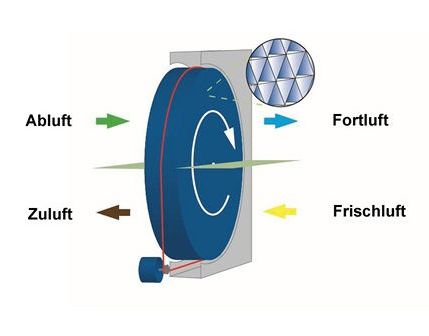
\includegraphics[width=0.49\textwidth]{Pictures/Rotation.jpg}}
	\subfigure[Membranbasierter Enthalpieübertrager]{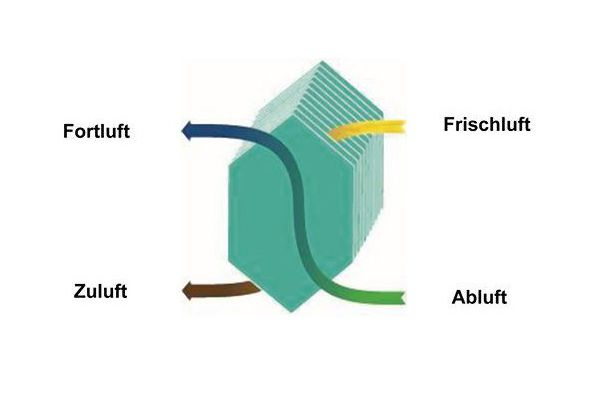
\includegraphics[width=0.49\textwidth]{Pictures/Enthalpieuebertrager.jpg}}
	\caption{Verschieden Ausführungsformen von Enthalpieübertragern}
	\label{fig:Enthalpieübertrager}
	
\end{figure}


Die Verbreitesten Speicherübertrager sind Rotationsübertrager. Rotationsübertrager weisen einen rotierende thermische Masse auf, die sich jeweils mit einem Teil der Masse im Zuluftstrom und mit einem anderen Teil der Masse im Abluftstrom befindet. Durch die Rotation kann die Masse thermische Energie in einem Luftstrom aufnehmen und nach dem Weiterrotieren im anderen Luftstrom abgeben. Analog funktioniert die Übertragung der Feuchte, wobei die Feuchte entweder von einem Sorptionsmaterial aufgenommen und wieder abgegeben wird oder in einem Luftstrom an der Masse kondensiert und im anderen Luftstrom wieder verdampft. Rotationsübertrager befinden sich bereits seit einigen Jahren kommerziell im Einsatz und wurden bereits entsprechend detailliert untersucht. %Quelle Bsp Performance comparisons of desiccant wheels for air dehumidification and enthalpy recovery
Membranbasierte Enthalpieübertrager sind erst seit wenigen Jahren kommerziell im Einsatz, sodass es bisher nur wenige Untersuchungen zu ihnen existieren. Die Wärme wird dann über die Membran von einem Luftstrom über an den anderen übertragen. Analog zum übertragenen Wärmestrom wird die Feuchte übertragen, das heißt Wasser wird vom Membranmaterial absorbiert, diffundiert durch die Membran und desorbiert auf der anderen Seite in den Luftstrom. Die Geometrien, die dabei für den Enthalpieübertrager verwendet werden, entsprechen denen, die bei klassischen Wärmeübertragern zum Einsatz kommen. In kommerziellen Anwendungen kommen Kreuzstromübertrager und Kreuzgegenstromübertrager zur Anwendung, wobei auch Gegenstromübertrager und "hollow fibre" Module mögliche Bauform darstellen. Kreuzstromübertrager sind im Vergleich zu Gegenstromübertragern Kostengünstig herstellbar und benötigen nur geringen Bauraum, daher sind sie die bisher häufigste Bauform bei Enthalpietauschern. Gegenstromübertrager haben im Gegensatz dazu einen hohen Wirkungsgrad. Deshalb hält vor allem eine Mischform aus beidem, der Kreuzgegenstromübertrager, immer stärker Einzug in die kommerzielle Nutzung. Hollow fibre Module ermöglichen hohe Übertragungsflächen bei kleinem Bauraum und somit hohe Übertragungsraten für Wärme und Feuchte. Nachteilig ist jedoch ein sehr hoher Druckverlust in den Modulen, der bisher verhindert hat, das diese Bauform sich in kommerziellen Anwendungen durchsetzen konnte. 

\begin{figure} [h]
	\centering
	%\includegraphics[width=400]{pictures/Vergleich_Geometirie.jpg}
	%\caption{Geometrien}
	%\label{fig:verschiendene Enthalpieübertrager-Geometrien}
	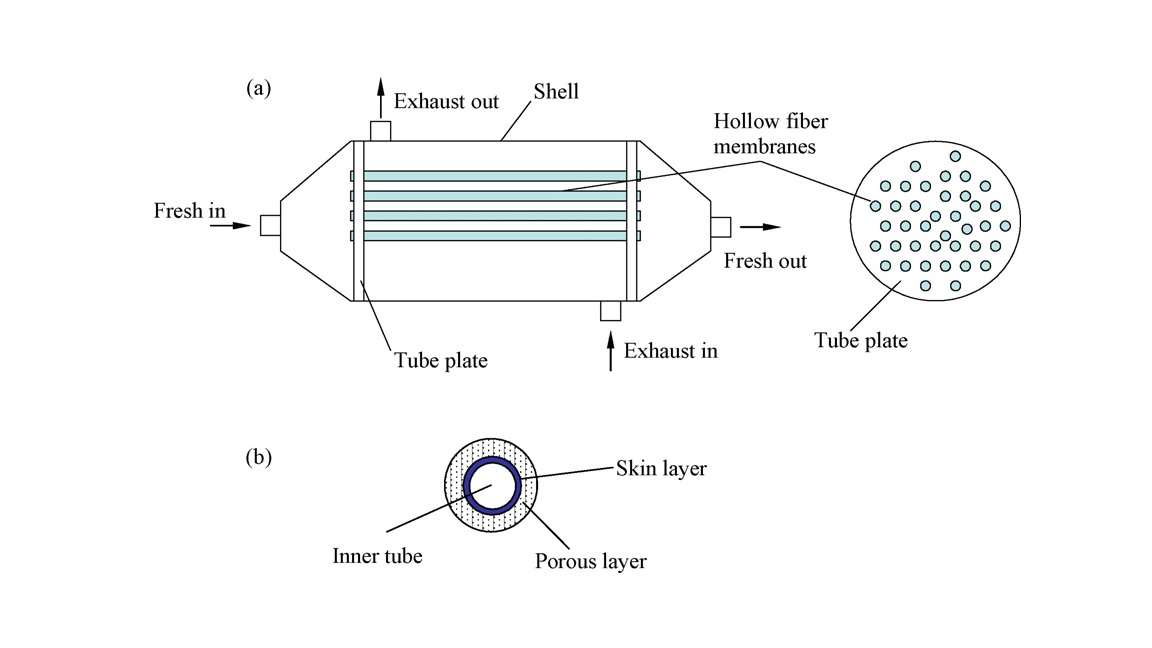
\includegraphics[width=0.98\textwidth]{pictures/hollow_fibre.jpg}
	\caption{hollow fibre}
	\label{fig:hollow fibre Modul}
\end{figure}

Ein Vergleich zwischen Rotationsübertragern und membranbasierten Enthalpietauschern fällt je nach Untersuchung unterschiedlich aus. Grundlegend haben jedoch membranbasierte Enthalpietauscher den Vorteil, dass sie keine beweglichen (rotierenden) Komponenten haben, was sie weniger verschleißanfällig macht und die Geräuschemissionen senkt. Außerdem muss keine Energie zum Antrieb eines Rotors aufgewendet werden. In den meisten Fällen besitzen membranbasierte Enthalpieübertrager den höheren Wirkungsgrad. %Quelle
Nachteilig ist, dass Enthalpieübertrager nicht regelbar sind. Laut % Quelle
ist es bei besonders feucht-warmen Tagen daher möglich, dass ein Enthalpieübertrager zur Feuchterückgewinnung der Zuluft zu viel Wasser zuführt. Dies könnte nur durch einen Bypass, eine Trockner oder einen Austausch des Enthalpieübertragers durch einen Wärmeübertrager für die entsprechende Jahreszeit verhindert werden. Außerdem können die membranbasierten Übertrager bei zu kalten Temperaturen zufrieren und müssen daher in einigen Klimazonen mit Vorheizern ausgestattet werden. Derzeit beherrschen Rotationsübertrager vor allem den Markt bei großen Anwendungsfällen während Enthalpieübertrager vor allem für Wohnungs- und Einzelraumlüftungen genutzt werden.  


\section{Membran}

Membranen lassen sich in dichte und poröse Membranen unterteilen. Poröse Membranen weisen Poren auf, die größer sind als die Partikel, die durch die Membran übertragen werden. Daher findet der Stofftransport aufgrund von.... statt. Dichte Membranen weisen hingegen keine oder nur sehr kleine Poren auf.  Der Stofftransport findet bei dichten Membranen auf Grund von Diffusionsprozessen statt. % evtl. noch sorption erwähnen
Dies führt in den meisten Fällen zu einer deutlich erhöhten Selektivität und einer geringeren Permeabilität im Vergleich zu porösen Membranen. Da im vorliegenden Anwendungsfall Wasserdampf als Permeat die Membran passieren soll und kleine gasförmige Moleküle der Luft, wie Stickstoff zurückgehalten werden sollen, ist eine Dichte Membran sinnvoll, da nur so eine ausreichende Selektivität gegenüber den gasförmigen Komponenten gewährleistet werden kann. Um dennoch eine möglichst hohe Permeabilität gegenüber Wasserdampf zu gewährleisten ist es zielführend eine möglichst dünne Membran zu verwenden. Um die dünnen dichten Membranen mechanische zu stabilisieren wird die dichte Membran in einigen Fällen durch eine poröse Membran gestützt. Die poröse Membran hat kaum negative Auswirkungen auf die Permeabilität, da die Transportgeschwindigkeiten in porösen Membranen wesentlichen höher sind als in dichten Membranen. Gleichzeitig ist jedoch anzunehmen, dass Spacermaterialien und porösen Membranen Einfluss auf die Strömung nehmen und somit auf die Wärmeübergangskoeffizienten und Sorptionseigenschaften an der Membranoberfläche. %auf wasseraffinität eingehen

\begin{figure} [h]
	\centering
	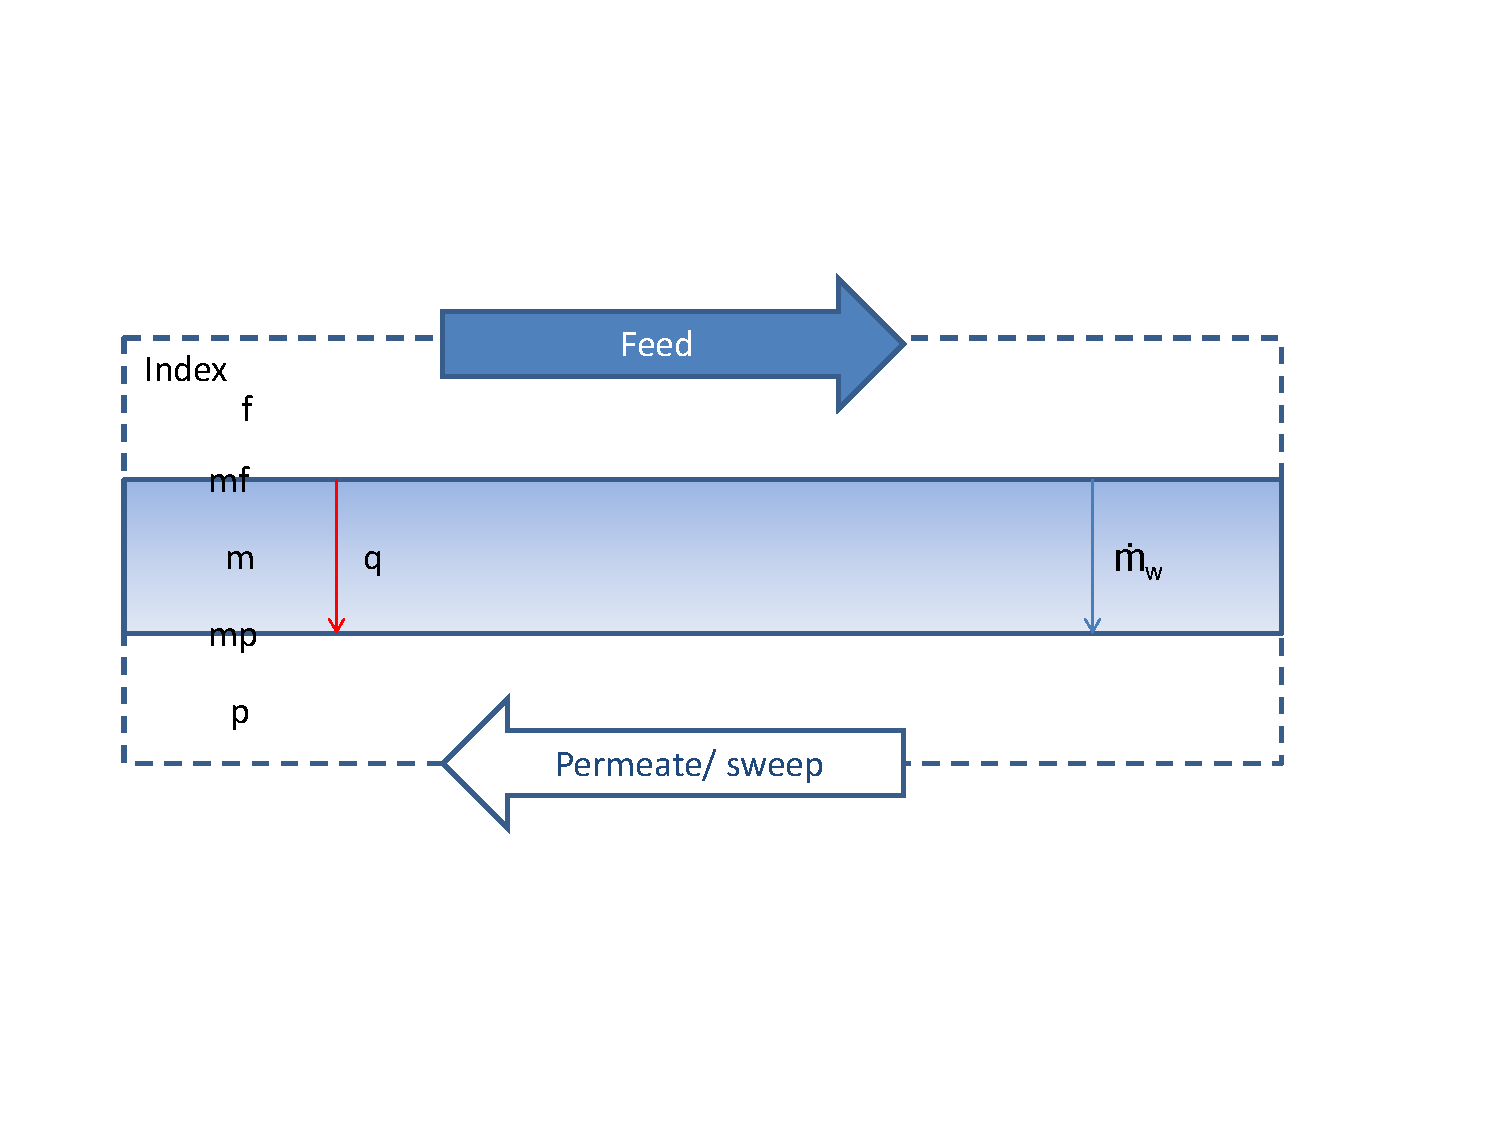
\includegraphics[width=0.98\textwidth]{pictures/Membran.pdf}
	\caption{Membran}
	\label{Membran}
\end{figure}

In Enthalpieübertragern werden derzeit Membranen aus Papier oder Polymeren eingesetzt. Die technische Weiterentwicklung der Polymermembranen über die letzten Jahre hat dazu geführt, das mittlerweile fast ausschließlich Polymermembranen zu Einsatz kommen, da diese deutlich höhere Permeabilitäten aufweisen. 

%Der Transport des Wasser von einem Luftstrom in den anderen Luftstrom durch die Membran lässt sich in 3 Phasen einteilen. Zuerst wird das Wasser auf einer Seite von der Membran Absorbiert, dann diffundiert das flüssige Wasser durch die Membran und wird auf der anderen Seite der Membran desobiert und an den Luftstrom abgegeben. 

% bild zum Transportprozess



Ein klassischer Vergleich über Wirkungsgrade, ist nur bedingt Sinnvoll. Die dabei bisher verwendeten Wirkungsgrade sind der Wärmeübertragungsgrad $\eta_{t}$ und der Enthalpiewirkungsgrad $\eta_{h}$. Der Wärmeübertragungsgrad hängt dabei rein von der thermischen Energie ab, 
%\begin{equation}

%\end{equation}.

Der Enthalpiewirkungsgrad beschreibt die gesamte übertragene Energie, also inklusive der Enthalpie die im übertragenen Wasserdampf steckt,
%\begin{equation}

%\end{equation}

Der Wärmeübertragungsgrad bei einem reine Wärmeübertrager ist fast immer größer, als bei einem Enthalipeübertrager und andersherum weißt der Enthalpieübertrager einen größeren gesamten Enthalpiewirkungsgrad auf.  Da membranbasierte Enthalpieübertrager ungeregelt Feuchte in den Zuluftstrom übertragen, ist die eine Bewertung anhand der Gesamtenthalpie oft nicht gerechtfertigt, da teilweise mehr feuchte übertragen wird als benötigt. %evtl. noch auf Normzustand und Abweichung über das Jahr eingehen
Der Wärmeübertragungsgrad stellt kein geeignetes Vergleichskriterium dar, da die übertragene Feuchte nicht berücksichtigt wird, die eine Hauptfunktion des Enthalpietauschers darstellt.




In dieser Arbeit sollen insbesondere membranbasierte Enthalpietauscher untersucht werden und Vergleichsgrößen die gefunden werden, die eine Energierückgewinnung mittels Enthalpietauschern mit anderen Systemen vergleichbar machen. Des Weiteren soll ein Modell der Enthalpieübertrager angefertigt werden, das zukünftig als Grundlage für Simulationen und für eine Weiterentwicklung der Modelle dienen soll, um Enthalpieübertrager auch in größeren Systemen simulativ einbinden zu können.  


\section{Stand der Technik}

Bisherige Veröffentlichungen zu Untersuchungen beschreiben vor allem Kennzahlermittlungen und die Genauigkeit bestimmter Modell-Ansätze. Für einen Überblick über die Veröffentlichungslage und den derzeitigen Stand der Technik empfehlen sich vor allem die Artikel....
Als Modelle werden vor allem Lösungs-Diffusions-Modelle vorgeschlagen. Sie beruhen auf der Annahme, dass Wasserdampf an der Oberfläche der Membran absorbiert wird, durch die Membran diffundiert und auf der gegenüberliegende Seite wieder an die Luft abgegeben wird. Aus dieser Betrachtungsweise ergeben sich verschiedene Möglichkeiten das System zu beschreiben. 
Grundsätzlich lassen sich die Publikationen in Bewertungs- beziehungsweise Komponentenoptimierungsorientierte und Modellermittelnde Untersuchungen unterteilen. Die bewertungsorientierten Arbeiten nutzen für den Vergleich verschiedener Bauweisen, Geometrien und Prinzipien vor bekannte Bewertungsgrößen wie die den Wärmeübertragungsgrad, die Feuchteübertragungsgrad oder den totalen Enthalpieübertragungsgrad. Sowie die Number of transfer units.
Bisherige Untersuchungen zur Modellbildung beziehen sich weitestgehend auf die Bestimmung Grundlegender Kenngrößen oder Beschreibungswerte die Analog zu bekannten Systemen definiert wurden. Hierbei kommen vor allem Größen zum Einsatz, die die unterschiedlichen für sich einzeln bereits bekannten Teilbereich der ablaufenden Prozesse in Beziehung zueinander setzt. So lassen sich  die Strömungseigenschaften, die Wärmeübertragung und die Feuchteübertragung getrennt voneinander betrachten und mit Kennzahlen, die ggf. von gewissen Parametern abhängen miteinander verknüpfen. Außerdem wurden in verschiedenen Artikeln unterschiedliche Annahmen überprüft beziehungsweise ihre Gültigkeit validiert. 

In dieser Arbeit soll im Gegensatz dazu ein Modell eines ermittelt werden das einen kommerziell einsatzfähigen Enthalpieübertrager beschreibt. Dabei liegt der Schwerpunkt nicht auf der Ermittlung der physikalischen Grundwerte oder Gültigkeit der physikalischen Modelle  und der zu Grunde liegenden Annahmen sondern auf der Beschreibung des Verhaltens des praktische eingesetzten Systems unter bestimmten Umgebungsbedingungen und in bestimmten Anwendungsfällen. Der Schwerpunkt liegt hier wiederum auf dem deutschen Klimaraum und dem Einsatz in Wohnraumlüftungen. 
%Die Betrachtungsweise bleibt also empirischer und und beschäftigt sich nicht mit den Materialeigenschaften
Ziel ist eine Modell zu generieren das Abhängig von Anforderungsprofilen und Umgebungsbedingungen eine Bewertung der Enthalpieübertragern insbesondere im Vergleich zu alternativen Systemen, wie z.B. Speicherenthalieübertragern und klassischen Wärmeübertragern mit entsprechender Lufttrocknung. Zu diesem Zweck sollen auch Bewertungsgrößen definiert werden die eine sinnvollen Vergleich der verschiedenen Größen zulassen. 




Enthalpieübertrager
Ein membranbasierter Enthalpietauscher nutzt die selektiven Eigenschaften einer Membran um einen Konzentrationsausgleich an Wasser zwischen den beiden Luftströmen auszugleichen. Dabei werden ansonsten die Funktionsweisen und Geometrien von klassischen Wärmeübertragern genutzt. Entsprechend lassen sich Kreuz-, Gegenstrom, Kreuz-Gegenstrom- und Gleichstrom Geometrien realisieren. Wobei die Kreuzstromgeometrie die am weitesten Verbreitete Geometrie ist, da sie die einfachste und kostengünstigste Version darstellt. Mit der Gegenstromgeometrie lässt sich der höchste Wirkungsgrad erreichen. Deshalb kommt auch diese Geometrie, sowie die Kreuz-Gegenstromgeometrie, als Kompromiss zwischen Gegenstrom- und Kreuzstromgeometrie, zum Einsatz. 
Ein weitere Unterscheidungskriterien sind der Anwendungsbereich, die Richtung des Feuchtetransports, die verwendete Membran,

Klassischer Anwenungsbereicht dieser Enthalpietauscher ist bisher die Einzelraumlüftung für Wohnungen und Büroräume. Aber auch größere Anwendungen sind mittlerweile möglich. Bisher liefern viele Anbieter die Lüftungsgeräte mit der Option aus den Enthalpietauscher im Sommer gegen einen Wärmeübertrager zu tauschen. Dies isst der Problematik geschuldet, dass die Enthalpieübertreager im Gegensatz zu den Rotationsübertragern nicht regelbar sind. Es besteht die Befürchtung, dass die im Sommer, wenn die Luftfeuchtigkeit in der Zuluft ohnehin hoch ist, eine weitere ungeregelte Anfeuchtung zu Schimmelbildung und Feuchteschäden führen kann. Hierzu gibt es in der Literatur verschiedene Ansichten. ...









Membranen sind bereits seit langem bekannt und kommen in technischen Bereichen bereits in vielen Gebieten zur Anwendung. Dabei unterliegen die ablaufenden Prozesse und Trennverfahren unterschiedlichen physikalischen Ursachen. In Enthalpieübertragern wird eine hohe Permeabilität der Membran gegenüber Wasser gefordert und eine geringe Permeabilität gegenüber verschiedene Gase, wie zum Beispiel Kohlenstoffdioxid und Stickstoff. Entsprechend werden in dieser Arbeit auch nur Membranen und Ihre physikalischen Grundlagen behandelt, die diese Eigenschaften erfüllen. Um eine ausreichende Isolierung gegen Gase zu erhalten ist es sinnvoll dichte Membranen zu nutzen. Naheliegend sind Membranen, die auf osmotischen Prinzipien beruhen. Osmotische Membranen werden bisher vor allem eingesetzt, um Wasser zu reinigen. 

 
\end{LARGE}
\end{normalsize}


\begin{table}[htb]
\centering
\caption{Das ist eine Testtabelle}\vspace{6pt}
\label{fig:PCM_Slurry1}
\begin{tabular}{cr} 
\hline
\textbf{Überschrift links} & \textbf{Überschrift rechts}\\
\hline 
links oben & rechts oben \\  
links unten & rechts unten \\ 
\hline 
\end{tabular}
\label{tab:Tabelle}
\end{table}


\chapter{Teil2}
\label{cha:Physikalische Grundlagen}



\begin{normalsize}


\section{Modell}
\label{sec:Modell}


\subsection{Stofftransport}

Die im untersuchten Enthalpieübertrager verwendete Membran besteht aus einer dichten Grundschicht und einer porösen Stützschicht. Der Stofftransport lässt sich analog zur Elektrotechnik als eine Kette von in Reihe geschalteten Prozessen darstellen. Eine Übersicht über die in Reihe geschalteten Prozesse gibt Abbildung\ref{fig:Transportprozesse}.
% Bild zu Membranprozessen einfügen

\begin{figure} [h]
	%\centering
	\caption{Transportprozesse}
	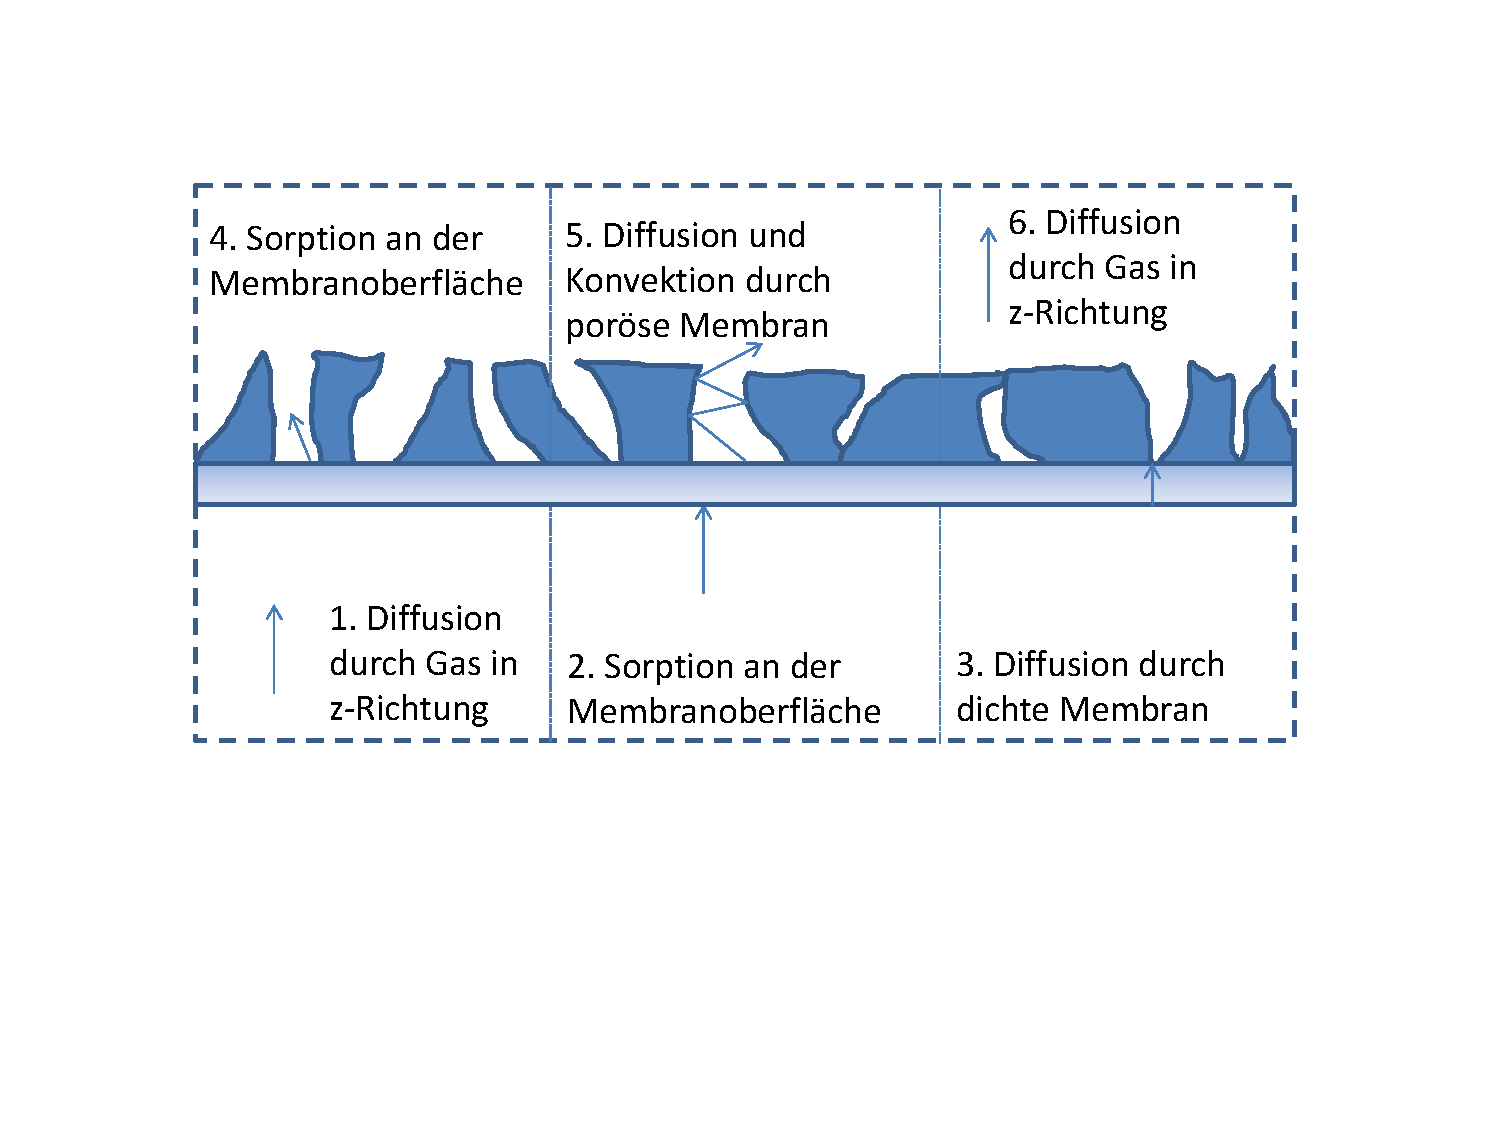
\includegraphics[width=0.98\textwidth]{pictures/Membran_Transportprozesse.pdf}
	
	\label{fig:Transportprozesse}
\end{figure}

Im ersten Schritt diffundiert der Wasserdampf durch den Luftstrom der Feedseite. Dies geschieht auf Grund eines Konzentrationsgradienten. Der Konzentrationsgradient entsteht durch das Ableiten des Wassermassenstroms durch die Membran. 

In einem zweiten Schritt absorbiert die Membranoberfläche den Wasserdampf. 

Im dritten Schritt folgt die Diffusion durch die dichte Grundschicht der Membran. 

Im vierten Schritt desorbiert das Wasser an der sweepseitigen Oberfläche der Membran in die Luft. 

In einem fünften Schritt wird der Wasserdampf durch die poröse Membran transportiert und verteilt sich in einem sechsten Schritt im Sweepstrom. Diese Diffusionsprozesse durch die Poren und den Luftstrom werden durch Konzentrationsgradienten verursacht.


Wie oben beschrieben führt die Betrachtung der 6 Prozessschritte als Reihenschaltung zu einer zutreffenden Beschreibung des Stofftransportes. Dies geschieht analog zur Elektrotechnik. Entsprechend ergibt sich der Gesamtwiderstand $W_{ges}$ der Membran 

\begin{equation}
 W_{ges} = W_{d} + W_{p}
\end{equation} 
 
aus einer Addition der Einzelwiderstände von dichter Membran $W_{d}$ und poröser Membran $W_{p}$.
 
Im Fall von parallel geschalteten Widerständen, zum Beispiel beim Auftreten von Poren in der dichten Membran, kann der Gesamtwiderstand analog zu 

\begin{equation}
\frac{1}{W_{ges}} = \frac{1}{W_{d}} + \frac{1}{W_{p}}
\end{equation}

gebildet werden. Beispiele hierfür sind das Auftreten von Poren in einer dichten Membran oder allgemein das parallele Stattfinden von konvektiven und diffusiven Stofftransportprozessen.


\subsubsection{Sorption an Membranoberfläche}
%Die Triebkraft des Sorptionsprozesses ist eine Differenz im chemischen Potential. Zur Beschreibung der Sorptionsprozesse werden meistens empirische und halbempirische Modelle genutzt. Das chemische Potential hängt im Fall der Sorption wesentlich von zwei Faktoren ab. Zum eine von der maximalen Wasserbeladung der Me
Die Triebkraft des Sorptionsprozesses ist eine Differenz im chemischen Potential. Meist werden hydrophile Membranenmaterialien für die dichte Membran eingesetzt. Daher entsteht an der Feed-Seite eine höherer Potentialdifferenz. Neben der Affinität des Membranmaterials ist die maximale Aufnahmekapazität der Membran ausschlaggebend für die Gleichgewichtskonzentration des Wassers in der Membranoberfläche. Dieses Lösungs-Gleichgewichtsmodell ist insbesondere von Lösungen anderer Aggregatzustände bekannt, z.B. von Salzlösungen oder Wasser-Luft-Lösungen. Die Beschreibung des Sorptionsprozesses mit physikalischen Modellen ist schwierig. Daher hat sich für die Beschreibung des Sorptionsprozesses ein halbempirisches Modell durchgesetzt, das sich in den meisten Veröffentlichungen wiederfindet, z.B. in \cite{J.L.Niu.2001} oder \cite{Dugaria.2015}. Demnach stellt sich in der Membranoberfläche eine Feuchtebeladung $\Theta$ von 

\begin{equation}
\Theta = \dfrac{\omega_{max}}{1-c+\frac{c}{\Phi}}
\end{equation}

ein. Wobei $\omega_{max}$ die maximal mögliche Feuchte im Membranmaterial angibt, $c$ eine Materialkonstante darstellt, die den Einfluss der Wasseraffinität der Membran wiederspiegelt, und $\Phi$ die Luftfeuchte im Luftstrom ist. 



\subsubsection{Diffusion durch dichte Membran}

Die Diffusion durch die dichte Membran ist im vorliegenden Fall der einflussreichste Prozessschritt auf die Transportgeschwindigkeit. Bei diesem Schritt ist der Widerstand am größten. Die Triebkraft ist hier - wie für alle Diffusionsprozesse - das chemische Potential. 
% ^ist das wirklich so?
%(Da die Wechselwirkungen mit der Temperatur gering sind und die es nicht zu relevanten chemischen Reaktionen kommt, kann der Partialdruck als Triebkraft angenommen werden. Im Fall von gleichem Druck auf beiden Seiten der Membran vereinfacht sich das System noch weiter und die Konzentration der Permeats in der Membranoberfläche kann als einzige relevante Triebkraft angesehen werden. 
%Daher resultiert der Permeatstrom J_{i} durch die Membran aus der Gleichung:
%\begin{equation}
%J_{i} = R*T*L_{i}/C_{i}*dC_{i}/dx
%\end{equation}

%in Abhängigkeit von der Gaskonstanten R, der Temperatur T und der Konzentration des Permeates i C_{i} und dessen örtlichen Gradienten dC_{i}/dx)

Unter der Annahme einer homogenen dichten Membran und konstanter thermodynamischer Randbedingungen (Druck und Temperatur) in der Membran ergibt sich eine lineare Konzentrationsverteilung über die Z-Achse der Membran. In der Literatur wird der Zusammenhang für den örtlichen Gradienten des chemischen Potentials und der übertragenen Stoffmenge ebenfalls als linear angenommen.(s.\cite{Koester.2015} 
%Literatur einfügen
%Da von konstanten thermodynamischen Eigenschaften in der Membran ausgegangen wird, ist es für die Modellierung egal ob der Massenstrom oder der Stoffmengenstrom betrachtet wird. 
Entsprechend ist für den Stoffmengentransport aus physikalischen Membranmodellen die Gleichung 

\begin{equation}
 \dot{n}^{\prime\prime} = - c_{wM} * b_{wM} * \frac{d\mu_{wM}}{dz}
\end{equation}

bekannt, wobei $\dot{n}^{\prime\prime}$ der Stoffmengenstrom des Wassers über die Membran ist und $b_{wM}$ die Beweglichkeit der diffundierenden Moleküle angibt. \cite{T.Melin.2007}
% hier: Nernst-Einstein, evtl noch auf Fick eingehen
Für den Diffusionsmassenstrom $J_{w}$ ergibt sich ein proportionaler Zusammenhang zum Gradienten des chemischen Potentials $\mu$

\begin{equation}
J_{w} = -L_{w}*\frac{d\mu_{w}}{dx}
\end{equation},

wobei $L_{w}$ der Proportionalitätsfaktor ist.

Das chemische Potential eines Stoffes $i$ ist definiert als Summe aus einem druckabhängigen Potentialterm, einem Standardpotentialterm und einem konzentrationsabhängigen Potentialterm zu

\begin{equation}
\mu_{i}(T,p,c_{i}) = \mu_{i}^\circ (T,p^\circ) + R*T*ln(a_{i}(T,p^\circ,c_{i})) + v_{i}*(p-p^\circ)
\end{equation},


wobei $P^\circ$ der Standarddruck ist, $R$ die ideale Gaskonstante \footnote{Gaskonstante = 8.314 J/mol/K}, $a_{i}$ die Aktivität des Stoffes $i$ und $v_{i}$ das Molvolumen des Stoffes $i$.


Der Druckterm
% würden sonst Einfluss auf die Durchmischung nehmen, da es die Geschw. d. Moleküle wiederspiegelt

\begin{equation}
v_{i}*(p-p^\circ)= 0
\end{equation}

entfällt unter der Voraussetzung einer idealen Gasmischung.

Der Standardpotentialterm $\mu_{i}^\circ(T,p^\circ)$ entfällt unter der Annahme von Isothermie entlang der z-Achse über die Membran. Da die dichte Membran sehr dünn ist, ist diese Annahme gerechtfertigt.
% Quellenangabe, evtl. Quelle 8 aber auch die Treffen eigentlich diese Annahme auch wenn sie Stoff und Wärmtransport koppeln wollen
% geringes delta T über mü, p0 auf beiden seiten gleich

Der konzentrationsabhängige Potentialterm hängt im Wesentlichen von der Aktivität der diffundierenden Komponente ab. Die Aktivität ist für Lösungen als
\begin{equation}
a_{i} = \gamma_{i}  * c_{i}
\end{equation}

definiert, wobei $\gamma_{i}$ der Aktivitätskoeffizient der Komponente $i$ ist. Der Aktivitätskoeffizient gibt das Verhältnis aus aktivem und realem Stoffmengenanteil an. Er nähert sich für kleine Konzentrationen dem Wert Eins. Da eine dichte Membran betrachtet wird, ist die Annahme sinnvoll.
Die oben beschriebenen Annahmen wurden auch von Zhang und Niu getroffen und mit experimentellen Ergebnissen validiert \cite{Zhang.2002b}. 

Aus den Annahmen folgt, dass der konzentrationsabhängige Potentialterm sich zu 

\begin{equation}
RT*ln(a_{i}(T,p^\circ,c_{i})) = RT*ln(c_{i})
\end{equation}

vereinfacht.

Unter den getroffenen Annahmen ergibt sich für den Stoffmengentransport von Wasser durch die Membran die Gleichung
%Detaillierter?
\begin{equation}
J_{w} = \frac{-L_{w}*RT}{c_{w}} * \frac{d c_{w}}{dx}
\end{equation}.

Daher lässt sich unter der Voraussetzung einer linearen Verteilung von $c_{w}$ über die z-Richtung der Membran ein linearer Zusammenhang des Stoffmengentransports von der Konzentrationsdifferenz mit einem Diffusionskoeffizienten $D_{w}$ beschreiben. So folgt die Gleichung:
\begin{equation}
J_{w} = D_{w} * \dfrac{c_{wfm}-c_{wsm}}{\delta}
\end{equation},

wobei $c_{wfm}$ und $c_{wsm}$ die Stoffmengenkonzentrationen in der feedseitigen beziehungsweise in der sweepseitigen Membranoberfläche darstellen.


\subsubsection{Diffusion durch poröse Membran}

Der Stofftransport durch die poröse Membran setzt sich aus einem Diffusionsprozess und einem Konvektionsprozess zusammen. Eine Konvektion in x- oder y-Richtung findet auf Grund der Porenausrichtung nicht statt. Die Konvektion in z-Richtung entsteht durch den Permeatstrom. Die Diffusion ergibt sich auf Grund des Konzentrationsgradienten. 

\subsubsection{Stofftransport im Luftstrom}

Bei der Beschreibung des Transports der Wassermoleküle durch die Gasphase führt die Annahme einer laminaren Luftströmung in x-Richtung zu einer deutlichen Vereinfachung des Modells. Im Fall laminarer Strömung kommt es nicht zum konvektiven Stoffaustausch in z-Richtung. Der Transport der Wassermoleküle in z-Richtung lässt sich unter dieser Annahme mit Hilfe von Diffusionsmodellen beschreiben.
Die Betrachtung turbulenter Stofftransportprozesse ist in der Regel mit aufwendigen Strömungssimulationen verbunden. Eine Beschränkung auf laminare Effekte kann somit den Rechenaufwand bei Simulationen erheblich reduzieren. 

Da die Turbulenz stark von der Geometrie  des Strömungskanals und der Strömungsgeschwindigkeit abhängt, ist diese Annahme nicht uneingeschränkt gültig. Insbesondere Spacermaterialien werden bewusst dazu eingesetzt, die Turbulenz in den Strömungskanälen zu erhöhen.
Eine erhöhte Turbulenz führt zu einer Abnahme der Konzentrationsüberhöhung an den Membranoberflächen und wirkt sich positiv auf die Sorptionsgeschwindigkeit an der Membranoberfläche aus.  

%Bild zur Konzentrationspolarisation einfügen
  
Konzentrationsüberhöhungen entstehen durch einen konvektiven Fluss. Der Permeatfluss durch die Membran zieht auf Grund der Kontinuitätsgleichungen einen konvektiven Massenstrom in z-Richtung nach sich. Da die Membran selektiv ist, diffundieren nur einige Stoffe, in diesem Fall die Wassermoleküle durch die Membran. Entsprechend nimmt die Konzentration der anderen Stoffe an der Membranoberfläche zu. Der Konzentrationsgradient des Wassers über die Membran ist daher geringer und somit auch die Triebkraft des Stofftransportes. Die Auswirkungen der Konzentrationspolarisation sind aber im hier betrachteten Fall gering, da der Permeatstrom im Vergleich zum Gesamtmassenstrom gering ist. 
%^noch mal prüfen und permeatstrom evtl. durch Diffusionsstrom o.Ä. ersetzen


\subsection{Zusammenfassend}


                                                                                               


\end{normalsize}


























 
%%%%%%%%%%%%%%%%%%%%%%%%%%%%%%%%%%%%%%%%%%%%%%%%%%%%%%%%%%%%%%%%%%%%%%%%%%%%%%%


%%%%%%%%%%%%%%%%%%%%%%%%%%%%%%%%%%%%%%%%%%%%%%%%%%%%%%%%%%%%%%%%%%%%%%%%%%%%%%%
% Einbinden der Bibliographie
% Das benötigte File liegt auf dem SVN-Server im Repository
% Nach Möglichkeit bitte dieses File verwenden, da es
% Mehrarbeit erspart!
%%%%%%%%%%%%%%%%%%%%%%%%%%%%%%%%%%%%%%%%%%%%%%%%%%%%%%%%%%%%%%%%%%%%%%%%%%%%%%%
\clearpage
\refstepcounter{Hilfszaehler}
\addcontentsline{toc}{chapter}{\bibname}
\protect\bibliographystyle{natdin}
\bibliography{Literatur1}
%%%%%%%%%%%%%%%%%%%%%%%%%%%%%%%%%%%%%%%%%%%%%%%%%%%%%%%%%%%%%%%%%%%%%%%%%%%%%%%


%%%%%%%%%%%%%%%%%%%%%%%%%%%%%%%%%%%%%%%%%%%%%%%%%%%%%%%%%%%%%%%%%%%%%%%%%%%%%%%
% Einbinden des Anhangs
%%%%%%%%%%%%%%%%%%%%%%%%%%%%%%%%%%%%%%%%%%%%%%%%%%%%%%%%%%%%%%%%%%%%%%%%%%%%%%%
\pagestyle{empty}
\clearpage
\vfill{}\vspace{-1\parskip}
\begin{center}\textsf{\textbf{\huge Anhang}}\end{center}{\huge \par}
\vfill{}
\appendix
\newpage
\pagestyle{fancy}
\chapter{Wichtiger Anhang 1}
Weit hinten, hinter den Wortbergen, fern der Länder Vokalien und Konsonantien leben die Blindtexte. Abgeschieden wohnen Sie in Buchstabhausen an der Küste des Semantik, eines großen Sprachozeans. Ein kleines Bächlein namens Duden fließt durch ihren Ort und versorgt sie mit den nötigen Regelialien. Es ist ein paradiesmatisches Land, in dem einem gebratene Satzteile in den Mund fliegen. Nicht einmal von der allmächtigen Interpunktion werden die Blindtexte beherrscht – ein geradezu unorthographisches Leben. Eines Tages aber beschloß eine kleine Zeile Blindtext, ihr Name war Lorem Ipsum, hinaus zu gehen in die weite Grammatik. Der große Oxmox riet ihr davon ab, da es dort wimmele von bösen Kommata, wilden Fragezeichen und hinterhältigen Semikoli, doch das Blindtextchen ließ sich nicht beirren.

\section{Die Versalien}
Es packte seine sieben Versalien, schob sich sein Initial in den Gürtel und machte sich auf den Weg. Als es die ersten Hügel des Kursivgebirges erklommen hatte, warf es einen letzten Blick zurück auf die Skyline seiner Heimatstadt Buchstabhausen, die Headline von Alphabetdorf und die Subline seiner eigenen Straße, der Zeilengasse. Wehmütig lief ihm eine rhetorische Frage über die Wange, dann setzte es seinen Weg fort. Unterwegs traf es eine Copy. Die Copy warnte das Blindtextchen, da, wo sie herkäme wäre sie zigmal umgeschrieben worden und alles, was von ihrem Ursprung noch übrig wäre, sei das Wort "und" und das Blindtextchen solle umkehren und wieder in sein eigenes, sicheres Land zurückkehren. Doch alles Gutzureden konnte es nicht überzeugen und so dauerte es nicht lange, bis ihm ein paar heimtückische Werbetexter auflauerten, es mit Longe und Parole betrunken machten und es dann in ihre Agentur schleppten, wo sie es für ihre Projekte wieder und wieder mißbrauchten.

Und wenn es nicht umgeschrieben wurde, dann benutzen Sie es immernoch. Weit hinten, hinter den Wortbergen, fern der Länder Vokalien und Konsonantien leben die Blindtexte. Abgeschieden wohnen Sie in Buchstabhausen an der Küste des Semantik, eines großen Sprachozeans. Ein kleines Bächlein namens Duden fließt durch ihren Ort und versorgt sie mit den nötigen Regelialien. Es ist ein paradiesmatisches Land, in dem einem gebratene Satzteile in den Mund fliegen. Nicht einmal von der allmächtigen Interpunktion werden die Blindtexte beherrscht – ein geradezu unorthographisches Leben. Eines Tages aber beschloß eine kleine Zeile Blindtext, ihr Name war Lorem Ipsum, hinaus zu gehen in die weite Grammatik. Der große Oxmox riet ihr davon ab, da es dort wimmele von bösen Kommata, wilden Fragezeichen und hinterhältigen Semikoli, doch das Blindtextchen ließ sich nicht beirren. Es packte seine sieben Versalien, schob sich sein Initial in den Gürtel und machte sich auf den Weg. Als es die ersten Hügel des Kursivgebirges erklommen hatte, warf es einen letzten Blick zurück auf die Skyline seiner Heimatstadt Buchstabhausen, die Headline von Alphabetdorf und die Subline seiner eigenen Straße, der Zeilengasse. Wehmütig lief ihm eine rhetorische Frage über die Wange, dann setzte es seinen Weg fort. Unterwegs traf es eine Copy. Die Copy warnte das Blindtextchen, da, wo sie herkäme wäre sie zigmal umgeschrieben worden und alles, was von ihrem Ursprung noch übrig wäre, sei das Wort "und" 

\chapter{Ähnlich wichtiger Anhang}
Es gibt im Moment in diese Mannschaft, oh, einige Spieler vergessen ihnen Profi was sie sind. Ich lese nicht sehr viele Zeitungen, aber ich habe gehört viele Situationen. Erstens: wir haben nicht offensiv gespielt. Es gibt keine deutsche Mannschaft spielt offensiv und die Name offensiv wie Bayern. Letzte Spiel hatten wir in Platz drei Spitzen: Elber, Jancka und dann Zickler. Wir müssen nicht vergessen Zickler. Zickler ist eine Spitzen mehr, Mehmet eh mehr Basler. Ist klar diese Wörter, ist möglich verstehen, was ich hab gesagt? Danke. Offensiv, offensiv ist wie machen wir in Platz. Zweitens: ich habe erklärt mit diese zwei Spieler: nach Dortmund brauchen vielleicht Halbzeit Pause. Ich habe auch andere Mannschaften gesehen in Europa nach diese Mittwoch. Ich habe gesehen auch zwei Tage die Training. Ein Trainer ist nicht ein Idiot! Ein Trainer sei sehen was passieren in Platz. In diese Spiel es waren zwei, drei diese Spieler waren schwach wie eine Flasche leer! Haben Sie gesehen Mittwoch, welche Mannschaft hat gespielt Mittwoch? Hat gespielt Mehmet oder gespielt Basler oder hat gespielt Trapattoni? Diese Spieler beklagen mehr als sie spielen! Wissen Sie, warum die Italienmannschaften kaufen nicht diese Spieler? Weil wir haben gesehen viele Male solche Spiel! Haben 
%%%%%%%%%%%%%%%%%%%%%%%%%%%%%%%%%%%%%%%%%%%%%%%%%%%%%%%%%%%%%%%%%%%%%%%%%%%%%%%


%%%%%%%%%%%%%%%%%%%%%%%%%%%%%%%%%%%%%%%%%%%%%%%%%%%%%%%%%%%%%%%%%%%%%%%%%%%%%%%
% Eigenständigkeitserklärung
%%%%%%%%%%%%%%%%%%%%%%%%%%%%%%%%%%%%%%%%%%%%%%%%%%%%%%%%%%%%%%%%%%%%%%%%%%%%%%%
\cleardoublepage
\pagestyle{empty}
\Large
\textsf{\textbf{Eigenständigkeitserklärung}}


\normalsize
\textsf{Hiermit versichere ich, dass ich die vorliegende Arbeit selbstständig und ohne Benutzung anderer als der angegebenen Hilfsmittel angefertigt habe. Alle Stellen, die wörtlich oder sinngemäß übernommen sind, sind als solche kenntlich gemacht. Die Arbeit ist in gleicher oder ähnlicher Form noch nicht als Prüfungsarbeit eingereicht worden. Ich erkläre mich damit einverstanden, dass die vorliegende Arbeit in der Lehrstuhlbibliothek und Datenbank aufbewahrt und für den internen Gebrauch kopiert werden darf.} \newline \newline


\textsf{Aachen, den \today \newline \newline}


\textsf{Name hier bitte einfügen}

%%%%%%%%%%%%%%%%%%%%%%%%%%%%%%%%%%%%%%%%%%%%%%%%%%%%%%%%%%%%%%%%%%%%%%%%%%%%%%%

\end{document}